% ============================================================
%  Presentació TFG — Web Core View
%  Autor: Jan Rosell Caba
%  Data:  Juny 2026
% ============================================================
\documentclass[aspectratio=169]{beamer}

% ---- Tema i colors (Estil Minimalista i Flat) ---------------
\usetheme{default}
\usecolortheme{default}

% Colors corporatius
\definecolor{upcblue}{RGB}{0, 82, 147}
\definecolor{upclight}{RGB}{240, 245, 250}
\definecolor{textdark}{RGB}{50, 50, 50}
\definecolor{accentgreen}{RGB}{37, 218, 117}
\definecolor{accentred}{RGB}{218, 37, 37}

% Configuració de la font i colors base
\setbeamercolor{normal text}{fg=textdark}
\setbeamercolor{structure}{fg=upcblue}
\setbeamercolor{alerted text}{fg=red!80!black}

% Eliminar els botons de navegació de baix a la dreta
\setbeamertemplate{navigation symbols}{}

% Títols de les diapositives
\setbeamertemplate{frametitle}{
    \vspace{0.4cm}
    {\Large\bfseries\color{upcblue}\insertframetitle}
    \par\vspace{0.1cm}
}

% Llistes amb punts discrets
\setbeamertemplate{itemize items}[circle]
\setbeamercolor{itemize item}{fg=upcblue}
\setbeamercolor{itemize subitem}{fg=upcblue!70}

% Estil dels blocs (Sense ombres i disseny pla)
\setbeamertemplate{blocks}[rounded][shadow=false]
\setbeamercolor{block title}{bg=upcblue, fg=white}
\setbeamercolor{block body}{bg=upclight, fg=textdark}
\setbeamercolor{block title alerted}{bg=red!80!black, fg=white}
\setbeamercolor{block body alerted}{bg=red!10, fg=textdark}
\setbeamercolor{block title example}{bg=accentgreen!70!black, fg=white}
\setbeamercolor{block body example}{bg=accentgreen!10, fg=textdark}

% Footer net i discret
\setbeamertemplate{footline}{
  \leavevmode%
  \hbox{%
  \begin{beamercolorbox}[wd=.333333\paperwidth,ht=3ex,dp=1.5ex,left,leftskip=2ex]{}%
    \textcolor{gray}{\small Jan Rosell Caba}
  \end{beamercolorbox}%
  \begin{beamercolorbox}[wd=.333333\paperwidth,ht=3ex,dp=1.5ex,center]{}%
    \textcolor{gray}{\small Web Core View}
  \end{beamercolorbox}%
  \begin{beamercolorbox}[wd=.333333\paperwidth,ht=3ex,dp=1.5ex,right,rightskip=2ex]{}%
    \textcolor{gray}{\small \insertframenumber{} / \inserttotalframenumber}
  \end{beamercolorbox}}%
  \vskip0pt%
}

% ---- Paquets ------------------------------------------------
\usepackage[utf8]{inputenc}
\usepackage[T1]{fontenc}
\usepackage[catalan]{babel}
\usepackage{graphicx}
\usepackage{booktabs}
\usepackage{pgfpages}
\usepackage{tikz}
\usepackage{eurosym}

% Activa les notes per a l'orador (comentar per a la versió final del PDF públic)
% \setbeameroption{show notes on second screen=right}

% ============================================================
\begin{document}

% ============================================================
% ===  BLOC 1: CONTEXT I PROBLEMA  ===
% ============================================================

% ---  DIAPOSITIVA 1 — Portada  ---
\begin{frame}[plain]
  \begin{center}
    \vspace{0.5cm}
    {\huge \bfseries \textcolor{upcblue}{Web Core View}}\\[0.4em]
    {\Large Modernització de la interfície web d'un NVR professional}\\[1.5em]

    {\large \textbf{Jan Rosell Caba}}\\[0.3em]
    {\small \textit{Director:} Fernando Gallego \quad|\quad \textit{Ponent:} Carles Farré}\\[0.2em]
    {\small Juny 2026}\\[1.5em]

    
\includegraphics[height=1.2cm]{../figures/logos/upc_complet.png}\hspace{0.8cm}
    
\includegraphics[height=1.2cm]{../figures/logos/fib_complet.png}\hspace{0.8cm}
    
\includegraphics[height=1.2cm]{../figures/logos/lanaccess_complet.png}
  \end{center}

  \note{
    Bon dia a tothom. El meu nom és Jan Rosell i avui presentaré el meu Treball de Fi de Grau: \textit{Web Core View}. Un projecte d'arquitectura web i modernització tecnològica per als gravadors de videovigilància professionals de Lanaccess.

    Tenim 20 minuts, així que aneu molt enrere, que la presentació serà dinàmica. Acabaré amb una demostració en vídeo de 5 minuts del sistema funcionant en viu.
  }
\end{frame}

% ---  DIAPOSITIVA 2 — Lanaccess i els NVR  ---
\begin{frame}{Lanaccess i els Gravadors NVR}
  \begin{columns}[T]
    \begin{column}{0.52\textwidth}
      \textbf{L'empresa}
      \begin{itemize}
        \item Lanaccess Telecom, SA: videovigilància professional.
        \item Producte estrella: família de gravadors \textbf{NXT}.
        \item Clients: empreses, institucions públiques, infraestructura crítica.
      \end{itemize}

      \vspace{0.5em}
      \textbf{El dispositiu}
      \begin{itemize}
        \item Fins a \textbf{152 càmeres} per unitat.
        \item SoC ARM (NXP i.MX), Linux Yocto.
        \item Desplegament \textit{standalone}: \textbf{sense Internet}.
      \end{itemize}
    \end{column}

    \begin{column}{0.44\textwidth}
      \begin{center}
        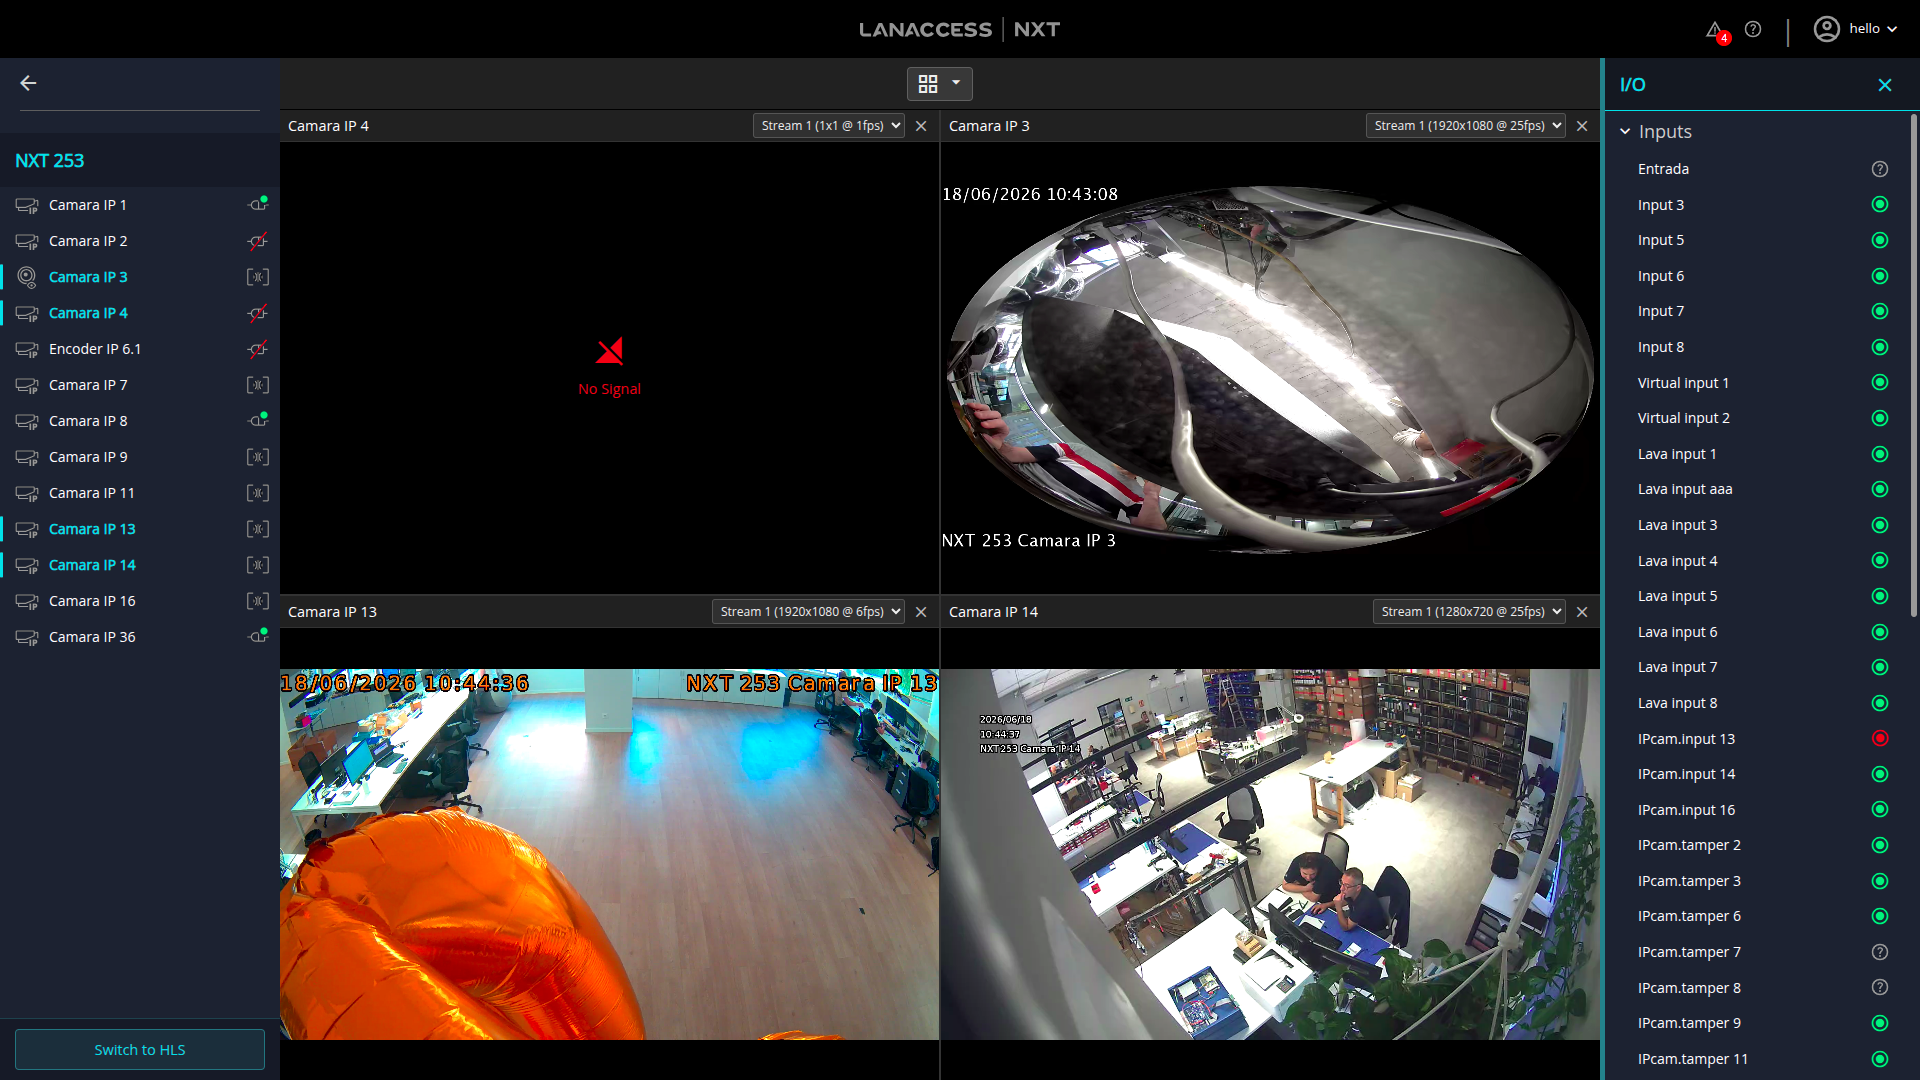
\includegraphics[width=\textwidth,keepaspectratio]{../figures/interficies/cameras.png}
      \end{center}
    \end{column}
  \end{columns}

  \note{
    Lanaccess és una empresa especialitzada en seguretat electrònica i videovigilància professional. El seu producte de referència és la família de gravadors NVR \textit{NXT}: dispositius que graven fins a 152 càmeres simultàniament. Funcionen sobre un processador ARM de NXP, corren Linux Yocto, i s'instal·len a les xarxes dels clients, que sovint no tenen sortida a Internet.

    Aquí hi ha la paraula clau: \textit{standalone}. Tot ha de funcionar sense dependre d'un servidor extern ni del núvol. L'NVR és l'únic servidor disponible.
  }
\end{frame}

% ---  DIAPOSITIVA 3 — El Problema: Fi d'una Era  ---
\begin{frame}{El Problema: La Fi d'una Era}
  \begin{columns}[T]
    \begin{column}{0.55\textwidth}
      \begin{alertblock}{L'herència: ActiveX (anys 90)}
        \begin{itemize}
          \item Plag dependent d'\textbf{Internet Explorer 11}.
          \item Microsoft tanca IE el \textbf{Juny 2022}.
          \item Incompatible amb macOS, Linux i mòbils.
          \item Vectors de seguretat documentats (OWASP).
        \end{itemize}
      \end{alertblock}

      \vspace{0.5em}
      \begin{itemize}
        \item Interfície estàtica: \textbf{sense reactivitat} ni temps real.
        \item Cada versió de firmware requeria canvis al frontend.
      \end{itemize}
    \end{column}

    \begin{column}{0.40\textwidth}
      \begin{block}{La pressió del mercat}
        \small Clients exigien accés des de qualsevol navegador i dispositiu modern.
      \end{block}

      \vspace{0.8em}
      \begin{block}{L'amenaça competitiva}
        \small Competidors amb interfícies web natives guanyaven terreny al catàleg NXT.
      \end{block}
    \end{column}
  \end{columns}

  \note{
    La situació de partida era crítica. Lanaccess tenia una plataforma web construïda als anys 90 basada en tecnologia ActiveX de Microsoft. El problema és que Internet Explorer 11, l'únic navegador que suportava ActiveX, va arribar al final de la seva vida el juny del 2022. I amb ell, va morir qualsevol possibilitat d'accedir als gravadors NXT des d'un Mac, un Linux, un mòbil, o simplement des de Chrome.

    A més, l'arquitectura era rígida: si el firmware canviava un paràmetre de configuració, un enginyer havia de modificar el frontend manualment. Això generava un deute tècnic creixent i una velocitat d'iteració molt lenta.

    La pressió del mercat era clara: els clients demandaven accés web modern, i la competència ja l'oferia.
  }
\end{frame}

% ---  DIAPOSITIVA 4 — L'Objectiu: Equip Autònom  ---
\begin{frame}{L'Objectiu: Un Sistema Web Autònom}

  \begin{center}
    \begin{tikzpicture}
      \node[draw=upcblue, rounded corners, fill=upclight, minimum width=2.5cm, minimum height=1.2cm, align=center] (browser) at (0,0) {\textbf{Navegador}\\\small Chrome/Firefox/Safari};
      \node[draw=upcblue, rounded corners, fill=upclight, minimum width=2.5cm, minimum height=1.2cm, align=center] (nvr) at (6,0) {\textbf{NVR NXT}\\\small Serveix tot};
      \draw[->, thick, upcblue] (browser.east) -- node[above]{\small HTTPS/WSS/WebRTC} (nvr.west);
    \end{tikzpicture}
  \end{center}

  \vspace{0.3em}
  \begin{columns}[T]
    \begin{column}{0.3\textwidth}
      \begin{exampleblock}{100\% Web}
        Cap plugin, cap instal·lació de client.
      \end{exampleblock}
    \end{column}
    \begin{column}{0.3\textwidth}
      \begin{exampleblock}{Autònom}
        L'NVR serveix l'app i el vídeo. Sense núvol.
      \end{exampleblock}
    \end{column}
    \begin{column}{0.3\textwidth}
      \begin{exampleblock}{Escalable}
        Nous firmwares no requereixen canvis al frontend.
      \end{exampleblock}
    \end{column}
  \end{columns}

  \note{
    L'objectiu del projecte es pot resumir en una frase: construir una aplicació 100\% web, basada en Angular 19, que s'executi de forma autònoma dins del propi gravador NVR, sense dependre de cap servidor extern ni plugin.

    Quan un operador obre el navegador i escriu la IP del gravador, l'NVR li serveix l'aplicació Angular, li ofereix els streams de vídeo i li envia les alarmes en temps real. Tot des del mateix dispositiu.

    I hi havia un tercer requisit diferencial: que l'aplicació fos escalable. Que si demà surten nous models de firmware amb noves opcions, el frontend s'adapti sol, sense que cap enginyer de software hagi de tocar el codi de la web.
  }
\end{frame}


% ============================================================
% ===  BLOC 2: LA SOLUCIÓ — ESPECIFICACIÓ  ===
% ============================================================

% ---  DIAPOSITIVA 5 — Els Actors del Sistema  ---
\begin{frame}{Els Actors del Sistema}
  \vspace{0.2em}
  \begin{columns}[T]
    \begin{column}{0.3\textwidth}
      \begin{block}{Administrador}
        \begin{itemize}
          \item[\small$\bullet$] Configuració completa.
          \item[\small$\bullet$] Gestió d'usuaris.
          \item[\small$\bullet$] Actualitzacions de firmware.
        \end{itemize}
      \end{block}
    \end{column}

    \begin{column}{0.3\textwidth}
      \begin{block}{Operador}
        \begin{itemize}
          \item[\small$\bullet$] Vídeo en directe.
          \item[\small$\bullet$] Gravacions i timeline.
          \item[\small$\bullet$] Gestió d'alarmes.
        \end{itemize}
      \end{block}
    \end{column}

    \begin{column}{0.3\textwidth}
      \begin{block}{Sistema NVR}
        \begin{itemize}
          \item[\small$\bullet$] Emet esdeveniments push.
          \item[\small$\bullet$] Dicta l'esquema JSON.
          \item[\small$\bullet$] Gestiona els \textit{config locks}.
        \end{itemize}
      \end{block}
    \end{column}
  \end{columns}

  \vspace{0.8em}
  \begin{center}
    \textbf{6 casos d'ús principals:} Autenticació $\cdot$ Vídeo directe $\cdot$ Gravacions $\cdot$ Alarmes $\cdot$ Configuració dinàmica $\cdot$ Administració
  \end{center}

  \note{
    L'anàlisi d'actors va revelar tres rols principals. L'Administrador té accés total: pot configurar el sistema, gestionar usuaris i actualitzar el firmware. L'Operador és el vigilant del dia a dia: veu les càmeres, revisa gravacions i gestiona alarmes. I el Sistema NVR actua com a tercer actor: és qui dicta les regles del joc mitjançant l'esquema JSON, qui emet els esdeveniments d'alarma, i qui gestiona els mecanismes de control d'accés a la configuració.

    A partir d'aquests actors vam derivar 6 casos d'ús principals que cobreixen tot el cicle de vida de la vigilància: autenticació segura, visualització de vídeo en directe, cerca de gravacions en una línia de temps, gestió d'alarmes, configuració dinàmica basada en esquema, i administració del sistema.
  }
\end{frame}

% ---  DIAPOSITIVA 6 — Requisits Crítics: Rendiment  ---
\begin{frame}{Requisits Crítics: Rendiment i Vídeo}
  \begin{columns}[T]
    \begin{column}{0.48\textwidth}
      \begin{alertblock}{RNF-01: Latència de vídeo}
        \begin{itemize}
          \item Objectiu: \textbf{$<$ 300 ms} de latència mitjana.
          \item P95: $<$ 350 ms.
          \item Motiu: sales de monitorització activa.
        \end{itemize}
      \end{alertblock}
    \end{column}

    \begin{column}{0.48\textwidth}
      \begin{alertblock}{RNF-03: Eficiència de CPU}
        \begin{itemize}
          \item Zero \textit{polling} HTTP.
          \item Actualitzacions granulars (\textit{Signals}).
          \item NGINX $\leq$ 5\% overhead addicional.
        \end{itemize}
      \end{alertblock}
    \end{column}
  \end{columns}

  \vspace{0.6em}
  \begin{columns}[T]
    \begin{column}{0.48\textwidth}
      \begin{block}{RNF-02: Fallback automàtic}
        Si UDP bloquejat: commuta a HLS en $\leq$ \textbf{5 segons}.
      \end{block}
    \end{column}

    \begin{column}{0.48\textwidth}
      \begin{block}{RNF-04: WebSocket resilient}
        Reconexió automàtica en $\leq$ \textbf{30 segons} (backoff exponencial).
      \end{block}
    \end{column}
  \end{columns}

  \note{
    Traduïm l'objectiu de negoci en requisits mesurables. El més crític és el de latència: en una sala de control de seguretat, si el vídeo va amb 2 segons de retard, una intrusió pot passar desapercebuda. Per això vam fixar 300 ms com a límit dur per al temps real.

    Igualment important és l'eficiència de CPU. L'NVR té una CPU ARM limitada. Si l'aplicació web consumeix massa processador al client, l'operador de vigilància veurà el seu PC aturats. Per això vam descartar qualsevol arquitectura basada en polling i vam apostar per actualitzacions push i reactivitat granular.

    I per cobrir les xarxes corporatives que bloquejen UDP —molt habituals en entorns industrials— vam especificar un fallback automàtic a HLS en menys de 5 segons.
  }
\end{frame}

% ---  DIAPOSITIVA 7 — Requisits Crítics: Seguretat  ---
\begin{frame}{Requisits Crítics: Seguretat i Privadesa}
  \begin{columns}[T]
    \begin{column}{0.48\textwidth}
      \textbf{Seguretat (OWASP Top 10)}
      \begin{itemize}
        \item Sense \textit{LocalStorage} per a credencials.
        \item Cookies \textbf{HttpOnly + Secure + SameSite}.
        \item Xifratge \textbf{TLS 1.2/1.3} i \textbf{WSS}.
        \item Immunitat XSS i CSRF per disseny.
      \end{itemize}
    \end{column}

    \begin{column}{0.48\textwidth}
      \textbf{Privadesa (RGPD / LOPDGDD)}
      \begin{itemize}
        \item \textbf{Privacy by Design}: dades sensibles només a RAM.
        \item Zero persistència al recarregar la pàgina.
        \item UNE-EN 62676: retenció 24h–30 dies.
        \item Sense emmagatzematge biometria.
      \end{itemize}
    \end{column}
  \end{columns}

  \vspace{0.6em}
  \begin{center}
    \begin{block}{}
      \centering La seguretat no és una capa afegida: és una \textbf{restricció de disseny} des del primer dia.
    \end{block}
  \end{center}

  \note{
    La seguretat en un sistema de videovigilància professional no és opcional. Estem tractant amb imatges de persones, dades sensibles, i infraestructura crítica. Per això vam imposar-nos el compliment de l'OWASP Top 10 com a criteri d'acceptació.

    La decisió més important va ser no emmagatzemar mai credencials al LocalStorage del navegador, que és accessible per qualsevol script de la pàgina. En el seu lloc, la sessió es gestiona amb cookies HttpOnly, que el navegador envia automàticament però que cap JavaScript pot llegir. Això elimina d'arrel els atacs de robatori de sessió per XSS.

    I per complir amb el RGPD, vam implementar el principi de Privacy by Design: si l'operador recarrega la pàgina, la sessió expira i les dades sensibles desapareixen de la memòria. Zero persistència per defecte.
  }
\end{frame}


% ============================================================
% ===  BLOC 3: LA SOLUCIÓ — DISSENY I ARQUITECTURA  ===
% ============================================================

% ---  DIAPOSITIVA 8 — Arquitectura Global  ---
\begin{frame}{Arquitectura Global del Sistema}
  \vspace{0.2em}
  \begin{columns}[T]
    \begin{column}{0.52\textwidth}
      \begin{center}
        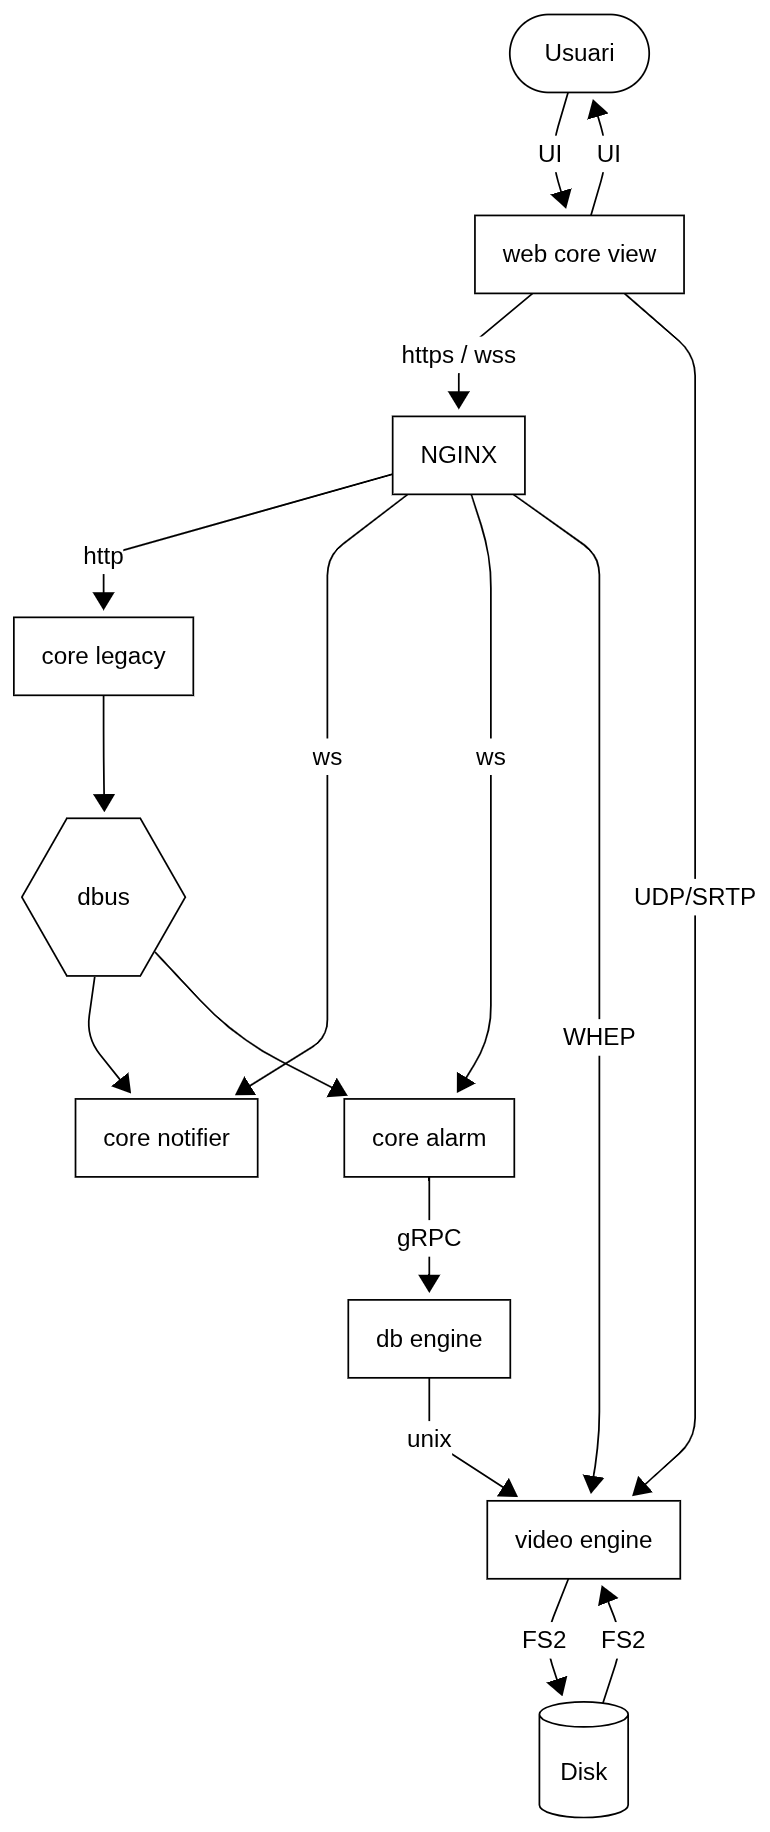
\includegraphics[width=\textwidth,keepaspectratio]{../figures/diagrames/arquitectura_serveis.png}
      \end{center}
    \end{column}
    \begin{column}{0.44\textwidth}
      \begin{itemize}
        \item \textbf{SPA:} Angular renderitza al navegador — allibera la CPU del gravador.
        \item \textbf{Microserveis C++:} cada procés gestiona un domini aïllat.
        \item \textbf{NGINX:} únic punt d'entrada, gestiona seguretat i routing.
      \end{itemize}
    \end{column}
  \end{columns}

  \note{
    El disseny arquitectònic respon directament als requisits de recursos limitats. En comptes d'un servidor monolític que tot ho processa, tenim una separació clara de responsabilitats.

    L'Angular és una Single-Page Application: es descarrega una vegada i s'executa completament al navegador del client. Això significa que el processament de la interfície, els càlculs de l'estat, les animacions, tot recau al PC de l'operador i no en la CPU del gravador.

    Al backend, cada responsabilitat és un procés C++ independent: un per a la configuració i autenticació, un per al motor de vídeo, un per a les alarmes. Aquesta separació permet que si el motor de vídeo falla, la configuració continuï funcionant.

    Entre els dos mons, NGINX actua com a porter: tota petició del navegador ha de passar per ell. Ell decideix a quin microservei la reenviar, gestiona el TLS i imposa les regles de seguretat.
  }
\end{frame}

% ---  DIAPOSITIVA 9 — Microserveis al Dispositiu  ---
\begin{frame}{Els Microserveis al Dispositiu}
  \vspace{0.2em}
  \begin{columns}[T]
    \begin{column}{0.48\textwidth}
      \begin{block}{Capa de comunicació}
        \begin{itemize}
          \item \texttt{la-core-legacy} — Config API, Auth.
          \item \texttt{la-db-engine} — SQLite via gRPC.
          \item \texttt{la-core-notifier} — Notificacions WSS.
          \item \texttt{la-core-alarm} — Alarmes WSS.
        \end{itemize}
      \end{block}
    \end{column}

    \begin{column}{0.48\textwidth}
      \begin{block}{Capa de vídeo}
        \begin{itemize}
          \item \texttt{la-video-engine} — Captura, disc, HLS.
          \item \texttt{MediaMTX} — WebRTC (WHEP) \& HLS.
          \item Sistema FS2: fitxers a bloc brut.
          \item Trans-muxing H.265 \textit{on the fly}.
        \end{itemize}
      \end{block}
    \end{column}
  \end{columns}

  \vspace{0.5em}
  \begin{itemize}
    \item Tots desplegats com a \textbf{unitats systemd} sobre Yocto Linux.
    \item Comunicació interna per \textbf{Unix Domain Sockets} i gRPC.
  \end{itemize}

  \note{
    Anem un nivell més avall per entendre quins processos corren dins del gravador. La capa de comunicació inclou el microservei de configuració i autenticació, el motor de base de dades que exposa SQLite via gRPC, i dos microserveis de WebSocket per a notificacions generals i alarmes específicament.

    La capa de vídeo és la més complexa: el la-video-engine s'encarrega de capturar les imatges de les càmeres, gravar-les al sistema de fitxers propietari FS2, i generar els segments de vídeo. MediaMTX és el servidor de streaming que gestiona tant les connexions WebRTC com el HLS.

    Tots aquests processos arrenen com a unitats systemd —el supervisor de processos de Linux— i es comuniquen internament sense passar per NGINX, evitant latències innecessàries. La comunicació entre la-db-engine i la-video-engine va per Unix Domain Sockets, que és la comunicació interprocessos més ràpida en Linux.
  }
\end{frame}

% ---  DIAPOSITIVA 10 — NGINX: Frontera de Seguretat  ---
\begin{frame}{NGINX: La Frontera de Seguretat}
  \begin{columns}[T]
    \begin{column}{0.55\textwidth}
      \textbf{Proxy invers i unificació}
      \begin{itemize}
        \item Un únic punt d'entrada: port \textbf{443 (HTTPS)}.
        \item Oculta ports interns dels microserveis.
        \item \textit{Routing}: \texttt{/stream/} $\to$ MediaMTX, \texttt{/ws/} $\to$ notificadors.
      \end{itemize}

      \vspace{0.4em}
      \textbf{Seguretat imposada}
      \begin{itemize}
        \item TLS 1.2/1.3 — Cifratge \textbf{AESGCM}.
        \item Cookies \textbf{HttpOnly + Secure + SameSite=Strict}.
        \item Cap script JavaScript pot llegir la sessió.
      \end{itemize}
    \end{column}

    \begin{column}{0.40\textwidth}
      \begin{alertblock}{Per què no JWT al LocalStorage?}
        \small Un XSS al navegador pot robar un token del LocalStorage. Una cookie HttpOnly és \textbf{invisible} per a qualsevol script de la pàgina.
      \end{alertblock}
    \end{column}
  \end{columns}

  \note{
    NGINX és molt més que un servidor web: és la nostra capa de seguretat per disseny. Primer, actua com a proxy invers unificant tots els serveis sota el port 443 amb HTTPS. Cap port intern dels microserveis és accessible directament des de l'exterior.

    Segon, i molt important, NGINX és qui gestiona les cookies de sessió. Quan un usuari s'autentica, NGINX genera una cookie amb els atributs HttpOnly i Secure. Això significa que el navegador l'envia automàticament a cada petició, però cap línia de JavaScript de l'aplicació Angular pot llegir-la ni modificar-la. Si un atacant injecta codi maliciós a la pàgina, no pot robar la sessió perquè mai hi té accés.

    Comparat amb la solució habitual de guardar un JWT al LocalStorage —que és trivial de robar per XSS— aquesta arquitectura elimina d'arrel la vulnerabilitat OWASP A07: Identification and Authentication Failures.
  }
\end{frame}

% ---  DIAPOSITIVA 11 — La Necessitat del Pessimistic Lock  ---
\begin{frame}{El Problema de la Concurrència en Configuració}
  \vspace{0.2em}
  \begin{center}
    \textit{Dos administradors editen simultàniament el mateix paràmetre de xarxa...}
  \end{center}

  \vspace{0.4em}
  \begin{columns}[T]
    \begin{column}{0.48\textwidth}
      \begin{alertblock}{Sense control de concurrència}
        \begin{enumerate}
          \small
          \item Admin A llegeix: \texttt{IP=192.168.1.50}
          \item Admin B llegeix: \texttt{IP=192.168.1.50}
          \item Admin A escriu: \texttt{IP=10.0.0.5}
          \item Admin B escriu: \texttt{IP=192.168.2.99}
          \item[\textbf{!}] \textbf{La configuració d'Admin A es perd.}
        \end{enumerate}
      \end{alertblock}
    \end{column}

    \begin{column}{0.48\textwidth}
      \begin{block}{La solució: Pessimistic Lock}
        \begin{itemize}
          \item Quan Admin A obre un mòdul, \textbf{adquireix el testimoni}.
          \item Admin B entra en \textbf{Mode Lectura} (\texttt{HTTP 423}).
          \item Cap escriptura simultània possible.
        \end{itemize}
      \end{block}
    \end{column}
  \end{columns}

  \note{
    En entorns de seguretat amb múltiples administradors, les col·lisions d'escriptura no són teòriques: ocorren. Imaginem dos tècnics que editen simultàniament la configuració de xarxa del gravador: canvien la IP del dispositiu. Sense cap mecanisme de control, s'aplicaria l'últim en escriure, i els canvis de l'altre s'esfumarien silenciosament, potencialment deixant el dispositiu en un estat inconsistent.

    En bases de dades, aquest problema es resol amb transaccions. En una interfície web multi-usuari, calia un mecanisme equivalent. Vam optar per un \textit{Pessimistic Lock}: quan un administrador obra un mòdul de configuració, el client demana un testimoni exclusiu al servidor. Qualsevol altre usuari que intenti editar el mateix mòdul rep una resposta HTTP 423 Locked i entra automàticament en mode de només lectura.
  }
\end{frame}

% ---  DIAPOSITIVA 12 — Disseny del Pessimistic Lock  ---
\begin{frame}{Disseny del \textit{Config Lock} Pessimista}
  \begin{columns}[T]
    \begin{column}{0.46\textwidth}
      \begin{center}
        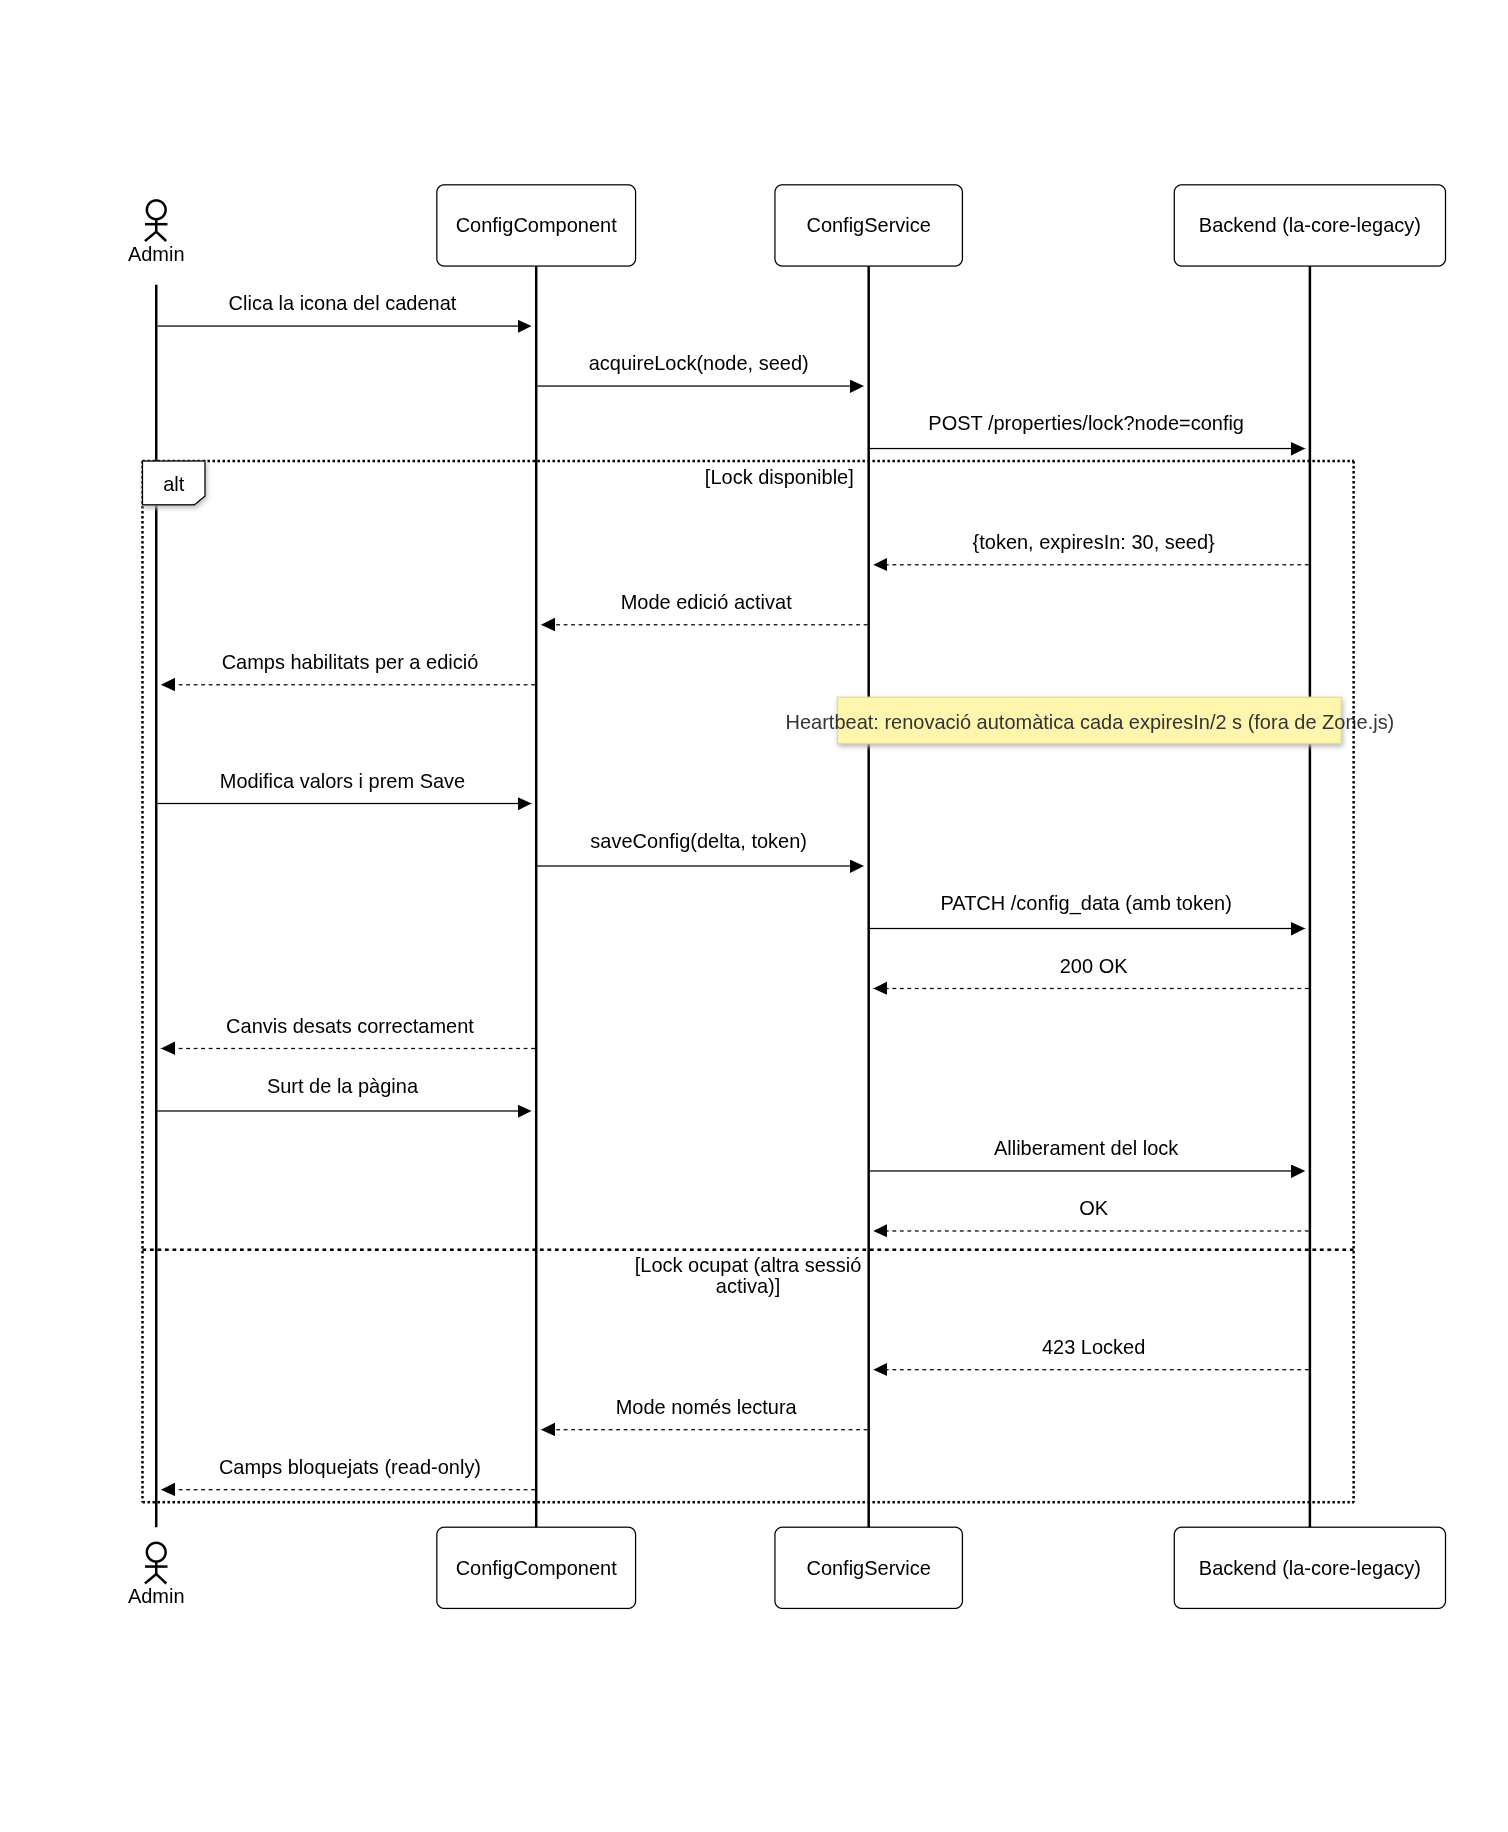
\includegraphics[width=\textwidth,keepaspectratio]{../figures/diagrames/seq_config_lock.png}
      \end{center}
    \end{column}

    \begin{column}{0.50\textwidth}
      \begin{itemize}
        \item \textbf{Adquisició:} POST \texttt{/lock} $\to$ token 32 hex.
        \item \textbf{Expiració:} \textbf{60--120 s} sense renovació.
        \item \textbf{Renovació automàtica:} fora del cicle d'Angular.
        \item \textbf{HTTP 423 Locked} $\to$ mode lectura per a altres.
      \end{itemize}

      \vspace{0.4em}
      \begin{block}{Tolerant a fallades}
        \small Talls de connexió $\Rightarrow$ el cadenat caduca sol. Cap procés queda bloquejat per sempre.
      \end{block}
    \end{column}
  \end{columns}

  \note{
    El disseny del Config Lock va requerir resoldre dos reptes oposats: que el lock fos segur però que no bloquegés indefinidament el sistema en cas de fallada.

    La seguretat es garanteix amb un token de 32 caràcters hexadecimals que cal enviar en cada petició d'escriptura. Si el token no coincideix o ha expirat, el servidor rebutja l'operació.

    La tolerància a fallades es garanteix amb l'expiració automàtica: si l'admin perd la connexió wifi, el torna a tancar el portàtil, o simplement tanca la pestanya sense alliberar el lock, el servidor no queda bloquejat per sempre. El cadenat expira als 60-120 segons i qualsevol altre administrador el pot adquirir.

    La renovació automàtica és transparent per l'usuari i, molt important, no passa pel cicle de detecció d'Angular. Hem implementat una crida HTTP a intervals regulars fora de la Zone.js, de manera que el keep-alive del lock no genera cap re-render innecessari de la interfície.
  }
\end{frame}


% ============================================================
% ===  BLOC 4: LA SOLUCIÓ — IMPLEMENTACIÓ  ===
% ============================================================

% ---  DIAPOSITIVA 13 — El Motor Schema-Driven  ---
\begin{frame}{El Cor del Projecte: Motor \textit{Schema-Driven}}
  \vspace{0.2em}
  \begin{center}
    \textit{El frontend no sap quantes càmeres ni quins paràmetres té el firmware. S'autoassembla en temps d'execució.}
  \end{center}

  \vspace{0.4em}
  \begin{columns}[T]
    \begin{column}{0.45\textwidth}
      \begin{block}{1. Backend dicta les regles}
        \small Envia un \textbf{JSON Schema} amb metadades:\\
        \texttt{\_type}, \texttt{\_allowedValues}, \texttt{\_min}, \texttt{\_max}, \texttt{\_default}
      \end{block}
    \end{column}

    \begin{column}{0.08\textwidth}
      \vspace{1.5em}\centering\large$\Rightarrow$
    \end{column}

    \begin{column}{0.45\textwidth}
      \begin{block}{2. Frontend renderitza}
        \small Angular genera automàticament \textit{inputs}, \textit{selects} i \textit{checkboxes} amb validació dinàmica nativa.
      \end{block}
    \end{column}
  \end{columns}

  \vspace{0.6em}
  \begin{exampleblock}{Impacte empresarial directe}
    Nou model de maquinari o opció de firmware $\Rightarrow$ \textbf{la interfície s'adapta sola}. Zero canvis al frontend.
  \end{exampleblock}

  \note{
    Aquí és on el projecte marca la diferència real per a Lanaccess. El motor Schema-Driven és la raó per la qual el frontend és firmwar-agnòstic.

    La idea és senzilla però poderosa: el backend no envia només dades, envia metadades. Quan el frontend demana la configuració de xarxa, el microservei respon amb un JSON que inclou no només els valors actuals, sinó també el tipus de cada camp (boolean, llista, IP, número), els valors permesos, els límits mínims i màxims, i els valors per defecte. Angular llegeix aquest esquema i renderitza el formulari complet de forma automàtica.

    L'impacte empresarial és enorme: si demà surt un nou model de NVR amb 20 paràmetres nous, o si el firmware exposa una nova opció de configuració, no cal tocar cap línia de codi del frontend. El C++ afegeix el camp a l'esquema JSON, i Angular el dibuixa sol.

    Això elimina el principal coll d'ampolla d'iteració del producte: la sincronia entre els equips de firmware i de frontend.
  }
\end{frame}

% ---  DIAPOSITIVA 14 — L'Esquema JSON en Acció  ---
\begin{frame}{L'Esquema JSON: De Metadades a Formulari}
  \begin{columns}[T]
    \begin{column}{0.50\textwidth}
      \textbf{Metadades del Backend (exemple)}
      \vspace{0.3em}
      \small
      \begin{tabular}{ll}
        \toprule
        \textbf{Clau} & \textbf{Valor} \\
        \midrule
        \texttt{ip\_address} & \texttt{"192.168.1.50"} \\
        \texttt{\_type} & \texttt{"ipaddr"} \\
        \texttt{\_description} & \texttt{"IP del dispositiu"} \\
        \midrule
        \texttt{codec} & \texttt{"H264"} \\
        \texttt{\_type} & \texttt{"list"} \\
        \texttt{\_allowedValues} & \texttt{["H264","H265"]} \\
        \midrule
        \texttt{max\_cameras} & \texttt{8} \\
        \texttt{\_type} & \texttt{"integer"} \\
        \texttt{\_min} & \texttt{1} \quad \texttt{\_max:} \texttt{152} \\
        \bottomrule
      \end{tabular}
    \end{column}

    \begin{column}{0.45\textwidth}
      \textbf{Frontend renderitza automàticament:}
      \vspace{0.3em}
      \begin{itemize}
        \item \texttt{ipaddr} $\to$ \textit{input} amb regex de validació IP.
        \item \texttt{list} $\to$ \texttt{<select>} amb les opcions permeses.
        \item \texttt{integer} $\to$ \textit{input number} amb rang [1, 152].
        \item \texttt{boolean} $\to$ \textit{checkbox}.
        \item \texttt{password} $\to$ camp amb política de seguretat.
      \end{itemize}
    \end{column}
  \end{columns}

  \note{
    Vegem com funciona el motor en la pràctica. La columna de l'esquerra és el que envia el microservei C++: un JSON amb els valors actuals i les metadades que comencen per guió baix. La columna de la dreta és el que renderitza Angular automàticament.

    Quan Angular detecta que el tipus és "ipaddr", genera un input de text amb una expressió regular que valida el format d'adreça IP. Quan veu "list" amb "allowedValues", genera un desplegable amb exactament aquelles opcions i cap altra. Quan veu "integer" amb min i max, genera un input numèric amb aquells límits ja configurats.

    El resultat és que un formulari de 50 camps es genera en mil·lisegons sense que cap enginyer de frontend hagi escrit cap component específic per a aquell cas. El motor té uns 10 tipus de camp que cobreixen el 100\% de la configuració del firmware.

    I quan el C++ afegeix un camp nou a l'esquema, Angular el veu la propera vegada que demana la configuració, i el renderitza sol. Sense deploy de frontend, sense PR, sense revisió de codi.
  }
\end{frame}

% ---  DIAPOSITIVA 15 — D'RxJS a Angular Signals  ---
\begin{frame}{L'Evolució de l'Estat: D'RxJS a Angular Signals}
  \begin{columns}[T]
    \begin{column}{0.48\textwidth}
      \textbf{L'antic paradigma (Zone.js + RxJS)}
      \begin{itemize}
        \item Cada event revisat \textbf{tot l'arbre} de components.
        \item 152 càmeres $\times$ alertes constants = CPU al límit.
        \item Un byte de canvi $\to$ el DOM s'escrutava sencer.
      \end{itemize}
    \end{column}

    \begin{column}{0.48\textwidth}
      \textbf{El nou paradigma (Angular 19 Signals)}
      \begin{itemize}
        \item Reactivitat \textit{fine-grained}: es repinta \textbf{només} el component afectat.
        \item Si un relé canvia d'estat $\to$ s'actualitza \textbf{una icona}.
        \item Zone.js eliminat del cicle crític.
      \end{itemize}
    \end{column}
  \end{columns}

  \vspace{0.8em}
  \begin{exampleblock}{\centering Resultat mesurat}
    \centering \textbf{35\% de reducció de CPU} al navegador en terminals de vigilància 24/7.
  \end{exampleblock}

  \note{
    L'arquitectura de gestió d'estat és una de les decisions tècniques que més impacte ha tingut en el rendiment final. Quan Angular va presentar els Signals a la versió 17 i els va estabilitzar al 19, vam decidir migrar completament.

    La diferència fonamental és que Zone.js funciona interceptant tots els events del navegador —clics, timers, peticions HTTP, WebSockets— i quan en detecta qualsevol, llança una revisió completa de l'arbre de components per saber si alguna cosa ha canviat. En una aplicació amb 152 càmeres, cada alerta WebSocket o cada keep-alive de sessió trigava una passada completa.

    Amb Signals, Angular sap exactament quins components depenen de quins valors. Quan el WebSocket emet un canvi d'estat d'un relé, Angular actualitza directament i exclusivament el component de la icona d'aquell relé. Un canvi puntual, una actualització puntual.

    El resultat mesurat en tests amb Intel Core i3-8100T: una reducció de CPU del 35\% en ús continu. Per a un operador que té la pantalla oberta 8 hores al dia, la diferència és substancial.
  }
\end{frame}

% ---  DIAPOSITIVA 16 — Orquestració de Vídeo: WebRTC  ---
\begin{frame}{Orquestració de Vídeo: WebRTC / WHEP (Directe)}
  \begin{columns}[T]
    \begin{column}{0.55\textwidth}
      \begin{block}{Protocol WebRTC via WHEP}
        \begin{itemize}
          \item Negociació SDP simplificada: HTTPS POST al \texttt{/stream/<cam>/whep}.
          \item Transport: \textbf{SRTP/UDP} + DTLS (RFC 3711).
          \item ICE per travessar NATs i tallafocs (RFC 8445).
        \end{itemize}
      \end{block}

      \vspace{0.5em}
      \begin{itemize}
        \item Latència mesura: \textbf{150--300 ms} en LAN.
        \item Fins a \textbf{4 càmeres} simultànies en mosaic.
      \end{itemize}
    \end{column}

    \begin{column}{0.40\textwidth}
      \begin{alertblock}{Per què WHEP i no WebRTC classic?}
        \small El WHEP (RFC 9716) estandarditza la negociació egress: una sola crida HTTP POST en lloc de l'ordinador SDP manual de WebRTC pur. Integra perfectament amb MediaMTX.
      \end{alertblock}
    \end{column}
  \end{columns}

  \note{
    El requisit de latència inferior a 300 ms imposava un protocol UDP. El candidat natural és WebRTC, però la seva implementació tradicional amb servidors de senyalització propis és complexa. Vam optar per WHEP, el WebRTC HTTP Egress Protocol, que és l'estàndard modern per a streaming de sortida.

    La negociació és molt elegant: el client Angular fa un simple POST HTTP a l'endpoint de l'stream de la càmera. El servidor respon amb el SDP de resposta. A partir d'aquí, s'estableix la connexió UDP directa amb xifrat DTLS per a la seguretat i ICE per a la travessia de NATs.

    El resultat pràctic és latències d'entre 150 i 300 mil·lisegons en xarxa local, amb una estabilitat molt alta. Comparat amb els 800-2000 ms de la plataforma ActiveX basada en RTSP, la millora és de 5 a 10 vegades.

    MediaMTX és el servidor d'streaming que implementa WHEP al costat del gravador, i integra molt bé amb el pipeline d'H.264 i H.265 de la capa de vídeo.
  }
\end{frame}

% ---  DIAPOSITIVA 17 — Orquestració de Vídeo: HLS  ---
\begin{frame}{Orquestració de Vídeo: HLS (Gravacions i Fallback)}
  \begin{columns}[T]
    \begin{column}{0.48\textwidth}
      \begin{block}{HLS per a gravacions (Timeline)}
        \begin{itemize}
          \item Transport sobre \textbf{TCP/HTTPS}: passa qualsevol tallafocs.
          \item Segmentos \texttt{.ts} servits per la-video-engine.
          \item Línia de temps interactiva amb seeks.
          \item Latència: \textbf{2--5 s} (acceptable per a playback).
        \end{itemize}
      \end{block}
    \end{column}

    \begin{column}{0.48\textwidth}
      \begin{block}{HLS com a fallback de directe}
        \begin{itemize}
          \item Si UDP bloquejat en $>$ \textbf{5 s}: commuta automàticament.
          \item El canvi és \textbf{transparent} per l'operador.
          \item Angular detecta timeout i re-negocia el protocol.
        \end{itemize}
      \end{block}
    \end{column}
  \end{columns}

  \vspace{0.5em}
  \begin{center}
    La dualitat WebRTC $\leftrightarrow$ HLS garanteix \textbf{cobertura universal} de xarxa sense comprometre la latència en LAN.
  \end{center}

  \note{
    HLS té dos rols en el sistema. El primer és el principal: és el protocol per a la visualització de gravacions. L'operador té una línia de temps interactiva on pot cercar qualsevol moment de les darreres hores o dies, i HLS serveix els segments de vídeo en ordre. Per a playback, 2-5 segments de retard és completament acceptable.

    El segon rol és el de fallback: en xarxes corporatives amb tallafocs estrictes, els ports UDP sovint estan tancats i WebRTC no pot establir connexió. En comptes de mostrar un error, Angular espera 5 segons i si no rep cap frame, commuta automàticament a HLS. L'operador potser nota uns 5 segments de latència addicional, però el vídeo apareix sense que hagi de fer res.

    Aquest disseny dual era un requisit de negoci important: molts clients de Lanaccess treballen en entorns corporatius amb tallafocs molt restrictius, i no podem dependre que els administradors de xarxa obrin ports UDP específics.
  }
\end{frame}

% ---  DIAPOSITIVA 18 — El Repte H.265  ---
\begin{frame}{El Repte H.265: Trans-muxing al Backend}
  \begin{columns}[T]
    \begin{column}{0.55\textwidth}
      \textbf{El problema}
      \begin{itemize}
        \item H.265 (HEVC): \textbf{50\% menys espai} que H.264 al disc.
        \item Molts navegadors restringeixen la descodificació H.265.
        \item Les gravacions FS2 estan en blocs bruts, sense contenidor.
      \end{itemize}

      \vspace{0.5em}
      \textbf{La solució: Trans-muxing}
      \begin{itemize}
        \item Llegir bloc brut de FS2.
        \item Injectar capçaleres SPS/PPS/VPS \textit{on the fly}.
        \item Empaquetar com a MPEG-TS per a HLS.
        \item \textbf{Sense recomprimir}: CPU intacta.
      \end{itemize}
    \end{column}

    \begin{column}{0.40\textwidth}
      \begin{exampleblock}{Trans-muxing vs Transcoding}
        \small \textbf{Transcoding:} descomprimir $+$ recomprimir. Alta CPU, alta qualitat.\\[0.5em]
        \textbf{Trans-muxing:} canviar contenidor, mantenir \textit{bitstream}. CPU quasi zero.
      \end{exampleblock}
    \end{column}
  \end{columns}

  \note{
    Aquesta va ser la desviació més gran del projecte: +25 hores extra per resoldre el repte de l'H.265.

    El context: els gravadors NVR utilitzen H.265 per emmagatzemar el vídeo perquè ocupa la meitat que H.264 per la mateixa qualitat. Però el problema és doble: els arxius estan en el sistema de fitxers propietari FS2, que escriu directament a blocs del disc sense cap contenidor estàndard. I quan intentes reproduir H.265 al navegador, Chrome i Firefox no el suportenten de forma universal.

    La solució que vam dissenyar és el trans-muxing: el microservei la-video-engine llegeix els blocs bruts de FS2, extreu les capçaleres SPS, PPS i VPS que contenen la informació de descodificació —que de vegades no estan en cada segment sinó que cal recuperar del keyframe anterior—, i les injecta davant del bitstream. Finalment, empaqueta tot en format MPEG-TS, que és el contenidor que entén HLS.

    La clau és que no estem recomprimint el vídeo, només canviem l'embolcall. Això significa que la CPU del gravador no s'ha d'esforçar en operacions de codificació, que serien molt costoses en un ARM embegut.
  }
\end{frame}

% ---  DIAPOSITIVA 19 — Alarmes en Temps Real  ---
\begin{frame}{Gestió d'Alarmes: WebSockets i SQLite VFS}
  \begin{columns}[T]
    \begin{column}{0.48\textwidth}
      \begin{block}{Persistència: SQLite + VFS Personalitzat}
        \begin{itemize}
          \item \textbf{remote\_vfs}: driver fet a mida.
          \item Escriptures via Unix socket: evita concurrència al disc.
          \item Sectors de \textbf{512 bytes}: atòmics davant talls de corrent.
          \item WAL mode: garanties ACID completes.
        \end{itemize}
      \end{block}
    \end{column}

    \begin{column}{0.48\textwidth}
      \begin{block}{Notificació: WebSockets Push}
        \begin{itemize}
          \item Zero \textit{polling}: connexió persistent WSS.
          \item Event push en \textbf{$<$ 1 s} al sensor.
          \item Sincronització entre tots els operadors: si un arxiva, tots ho veuen.
          \item Reconexió automàtica amb backoff exponencial.
        \end{itemize}
      \end{block}
    \end{column}
  \end{columns}

  \note{
    El sistema d'alarmes requeria resoldre dos problemes independents: la persistència fiable i la notificació en temps real.

    Per a la persistència, la restricció era dura: el gravador pot patir talls de corrent sobtats, i cap alarma de seguretat pot perdre's en aquell moment. SQLite amb el mode WAL ofereix garanties ACID, però la seva configuració per defecte no és òptima per a escritps moltes concurrents en un sistema embegut. El VFS personalitzat, remote_vfs, redirigeix totes les operacions de disc a través d'un Unix Domain Socket cap al la-video-engine, que és l'únic procés amb permisos d'escriptura al disc. Les escriptures s'alineen a sectors de 512 bytes per garantir atomicitat.

    Per a la notificació, vam substituir el clàssic polling HTTP —preguntar al servidor cada 2 o 5 según si hi ha alarmes noves— per WebSockets bidireccionals. Quan un sensor d'intrusió salta, el la-core-alarm ho rep, ho persists a SQLite i ho envia immediatament per WebSocket a tots els operadors connectats. No hi ha polling, no hi ha latència artificial, i si un operador arxiva l'alarma, tots els altres ho veuen reflectit en temps real.
  }
\end{frame}


% ============================================================
% ===  BLOC 5: PROVES I VALIDACIÓ  ===
% ============================================================

% ---  DIAPOSITIVA 20 — Validació: Latència  ---
\begin{frame}{Validació: Latència — ActiveX vs WebRTC}
  \vspace{0.3em}
  \begin{columns}[T]
    \begin{column}{0.55\textwidth}
      \begin{center}
        \renewcommand{\arraystretch}{1.4}
        \begin{tabular}{lcc}
          \toprule
          \textbf{Protocol} & \textbf{Latència} & \textbf{Estabilitat} \\
          \midrule
          ActiveX + RTSP (legacy) & 800--2000 ms & Baixa \\
          \textbf{WebRTC / WHEP} & \textbf{150--300 ms} & Alta \\
          HLS (fallback) & 2--5 s & Molt alta \\
          \bottomrule
        \end{tabular}
      \end{center}

      \vspace{0.5em}
      \textbf{Millora:} \textbf{5--10$\times$} menys latència que la plataforma legacy.
    \end{column}

    \begin{column}{0.40\textwidth}
      \begin{exampleblock}{RNF-01 assolit}
        \centering $<$ 300 ms de latència amb WebRTC. $<$ 350 ms P95.\\[0.4em]
        \small Validat en xarxa LAN amb Intel i3-8100T com a client.
      \end{exampleblock}
    \end{column}
  \end{columns}

  \note{
    Els resultats de latència superen les expectatives. Amb WebRTC en xarxa local, hem obtingut una latència d'entre 150 i 300 mil·lisegons, que és fins a 10 vegades millor que la plataforma ActiveX basada en RTSP, que oscil·lava entre 800 ms i 2 segments.

    L'origen de la millora és estructural: ActiveX usava RTSP sobre TCP, que afegeix overhead de control de flux i retransmissions. WebRTC fa servir UDP amb SRTP, on cada paquet va pel camí més ràpid i no espera confirmació dels anteriors. La latència de percepció en sala de control ha passat de "clarament visible" a "pràcticament imperceptible".

    El fallback HLS té 2-5 segments de latència, cosa que és completament acceptable per a visualitzar gravacions. Per a directe en xarxes restrictives, és menys ideal però garanteix que sempre hi ha imatge.

    El requisit RNF-01 és complert amb marge.
  }
\end{frame}

% ---  DIAPOSITIVA 21 — Validació: CPU i Usabilitat (SUS)  ---
\begin{frame}{Validació: Rendiment i Usabilitat}
  \begin{columns}[T]
    \begin{column}{0.48\textwidth}
      \begin{block}{Eficiència de CPU (Signals)}
        \begin{itemize}
          \item \textbf{35\% de reducció} de CPU al client.
          \item Zero fuites de memòria (streaming 2h validat).
          \item Rang estable: 45--65 MB de RAM.
          \item Neteja correcta del \texttt{RTCPeerConnection}.
        \end{itemize}
      \end{block}
    \end{column}

    \begin{column}{0.48\textwidth}
      \begin{block}{Test d'Usabilitat SUS}
        \begin{itemize}
          \item \textbf{Puntuació: 85.6 / 100} (categoria \textit{Excel·lent}).
          \item 8 participants: tècnics i operadors reals.
          \item Benchmark: $>$80 = Bo, $>$70 = Acceptable.
          \item Firmwares actualitzats un \textbf{40\% més ràpid}.
        \end{itemize}
      \end{block}
    \end{column}
  \end{columns}

  \vspace{0.5em}
  \begin{exampleblock}{\centering Tots els RNF tècnics i d'usabilitat: assolits}
    \centering WS reconnecta en $\leq$ 30 s $\cdot$ 25 connexions concurrents $\cdot$ zero corrupció VFS en talls de corrent
  \end{exampleblock}

  \note{
    Passem als resultats de rendiment i usabilitat. En termes de CPU, la migració a Signals ha donat una reducció del 35\% de consum computacional al navegador. I en el test de streaming WebRTC de dues hores, no s'han detectat fuites de memòria: la memòria oscil·la de forma saludable entre 45 i 65 MB amb el garbage collector de V8 fent el seu treball.

    Per a la usabilitat, vam aplicar el System Usability Scale, el test de referència en enginyeria de software. Amb 8 participants —tècnics d'instal·lació i operadors de seguretat reals— hem obtingut 85.6 sobre 100, que entra a la categoria d'Excel·lent. El punt de referència és que 70 és "acceptable" i 80 és "bo". La nostra puntuació és per sobre de les dues.

    Destaca especialment la dada dels firmwares: els tècnics van ser capaços d'actualitzar el firmware en un 40\% menys de temps que amb la plataforma legacy, gràcies a la interfície guiada i al sistema de validació en temps real.

    En resum: tots els requisits no funcionals estan validats amb dades.
  }
\end{frame}


% ============================================================
% ===  BLOC 6: DEMOSTRACIÓ  ===
% ============================================================

% ---  DIAPOSITIVA 22 — Demo  ---
\begin{frame}[plain]
  \begin{center}
    \vspace{2em}
    {\Huge \bfseries \textcolor{upcblue}{Demostració del Sistema}}\\[1em]
    {\large Vídeo de 5 minuts: el sistema en funcionament real}\\[2em]

    \begin{tikzpicture}
      \draw[upcblue, line width=2pt, rounded corners=8pt] (0,0) rectangle (8,4.5);
      \node at (4,2.25) {\textcolor{upcblue!40}{\Huge $\blacktriangleright$}};
      \node[below] at (4,0.3) {\small \textcolor{gray}{Web Core View — NVR NXT en viu}};
    \end{tikzpicture}
  \end{center}

  \note{
    Aquí és on farem una pausa per reproduir el vídeo de demostració. El vídeo mostra:

    1. Autenticació segura i login al sistema.
    2. El mosaic de 4 càmeres en directe via WebRTC: latència visible en temps real.
    3. La línia de temps interactiva per a la cerca de gravacions en HLS.
    4. La gestió d'alarmes amb el push via WebSocket: un sensor salta i la UI s'actualitza instantàniament.
    5. El motor Schema-Driven en acció: la pàgina de configuració que es genera automàticament a partir de l'esquema JSON del firmware.

    Recordeu que tot el que veieu s'executa dins del gravador NVR, sense cap servidor extern ni connexió a Internet.
  }
\end{frame}


% ============================================================
% ===  BLOC 7: ASPECTES TRANSVERSALS  ===
% ============================================================

% ---  DIAPOSITIVA 23 — Planificació i Desviacions  ---
\begin{frame}{Planificació: Desviacions i Gestió del Risc}
  \begin{columns}[T]
    \begin{column}{0.55\textwidth}
      \renewcommand{\arraystretch}{1.3}
      \begin{tabular}{lcc}
        \toprule
        \textbf{Fase} & \textbf{Previst} & \textbf{Executat} \\
        \midrule
        Gestió i Formació & 40 h & 40 h \\
        Auth \& Core & 60 h & 60 h \\
        Manteniment Base & 70 h & 70 h \\
        Alarmes \& Vídeo & 120 h & \textbf{145 h} \\
        Gravacions \& Config & 170 h & \textbf{190 h} \\
        Finalització & 80 h & 80 h \\
        \midrule
        \textbf{Total} & \textbf{540 h} & \textbf{585 h} \\
        \bottomrule
      \end{tabular}
    \end{column}

    \begin{column}{0.40\textwidth}
      \textbf{Causes de la desviació (+45 h):}
      \begin{itemize}
        \item H.265: SPS/PPS/VPS injection $\to$ \textbf{+25 h}.
        \item Motor Schema-Driven $\to$ \textbf{+20 h}.
      \end{itemize}

      \vspace{0.5em}
      \begin{exampleblock}{Resultat}
        \small Desviació absorbida dins del \textbf{10\% de contingència} previst. Cap feita tallada.
      \end{exampleblock}
    \end{column}
  \end{columns}

  \note{
    La planificació del projecte va ser bastant precisa en la majoria de fases. Les desviacions es van concentrar en dos punts, que curiosament coincideixen amb les dues aportacions tècniques més innovadores del projecte.

    La primera desviació de 25 hores va ser la integració de l'H.265. Inicialment estimàvem que bastaria amb canviar el contenidor, però la realitat del sistema de fitxers FS2 —que no desa les capçaleres SPS/PPS/VPS en cada segment— va requerir un algorisme de recuperació de capçaleres des del keyframe anterior. Això no estava previst i va ser complexe.

    La segona desviació de 20 hores va ser el disseny del motor Schema-Driven. A mesura que avançàvem, vam adonar-nos que el nombre de tipus de camp necessaris era superior a l'estimat —llistes dinàmiques, camps condicionats, adreces IP en formats múltiples. Va valer la pena cada hora extra.

    En total, +45 hores sobre les 540 previstes: un 8.3\% de desviació, que cau perfectament dins del marge de contingència del 10\% que havíem reservat. El resultat és que cap funcionalitat va ser retallada ni ajornada.
  }
\end{frame}

% ---  DIAPOSITIVA 24 — Pressupost  ---
\begin{frame}{Pressupost: Cost Previst vs Executat}
  \vspace{0.3em}
  \begin{columns}[T]
    \begin{column}{0.55\textwidth}
      \renewcommand{\arraystretch}{1.3}
      \begin{tabular}{lcc}
        \toprule
        \textbf{Partida} & \textbf{Previst} & \textbf{Executat} \\
        \midrule
        Personal (hores) & 13.567,50 \euro & 14.701,50 \euro \\
        Amortització HW & 210,00 \euro & 210,00 \euro \\
        Costos indirectes & 1.150,00 \euro & 1.150,00 \euro \\
        Contingència (10\%) & 1.492,75 \euro & 1.134,00 \euro \\
        \midrule
        \textbf{Total} & \textbf{16.420,25 \euro} & \textbf{16.061,50 \euro} \\
        \bottomrule
      \end{tabular}
    \end{column}

    \begin{column}{0.40\textwidth}
      \begin{exampleblock}{\centering Estalvi net}
        \centering \textbf{358,75 \euro} per sota del pressupost.\\[0.4em]
        \small La contingència s'ha usat parcialment (76\%), no al 100\%.
      \end{exampleblock}

      \vspace{0.5em}
      \begin{block}{Perfil de cost}
        \small $>$90\% és cost de personal. El HW és amortitzat de maquinari de desenvolupament existent.
      \end{block}
    \end{column}
  \end{columns}

  \note{
    El pressupost final és de 16.061 euros, per sota dels 16.420 euros previstos. Com veiem a la taula, el cost de personal va pujar degut a les 45 hores extra, però la contingència que havíem reservat no va caldre consumir-la completament.

    El perfil de costos és el típic d'un projecte de software: més del 90% del cost és personal. El maquinari és amortització d'equipament de desenvolupament existent i representa una fracció petita.

    Cal destacar que la contingència s'ha usat de forma parcial —el 76%— per cobrir les desviacions de les fases de vídeo i configuració. Que no s'hagi exhaurit completament és un bon indicador de gestió: la contingència existeix per ser usada davant de riscos materialitzats, no per ser conservada com un trofeu.

    El projecte ha entregat tot l'abast previst, a temps, i per sota del pressupost màxim.
  }
\end{frame}

% ---  DIAPOSITIVA 25 — Sostenibilitat  ---
\begin{frame}{Sostenibilitat i Impacte Social}
  \begin{columns}[T]
    \begin{column}{0.3\textwidth}
      \begin{block}{Ambiental}
        \begin{itemize}
          \item[\small$\bullet$] 35\% menys CPU $\to$ menys consum elèctric.
          \item[\small$\bullet$] Gestió remota $\to$ menys desplaçaments de tècnics.
          \item[\small$\bullet$] Hardware existent reutilitzat.
        \end{itemize}
      \end{block}
    \end{column}

    \begin{column}{0.3\textwidth}
      \begin{block}{Social}
        \begin{itemize}
          \item[\small$\bullet$] UI clara redueix estrès en torns 24/7.
          \item[\small$\bullet$] Accessibilitat multiplataforma (Linux, Mac).
          \item[\small$\bullet$] Privadesa per disseny (RGPD).
        \end{itemize}
      \end{block}
    \end{column}

    \begin{column}{0.3\textwidth}
      \begin{block}{Econòmica}
        \begin{itemize}
          \item[\small$\bullet$] Schema-driven: zero cost per nou firmware.
          \item[\small$\bullet$] PWA futura: diagnòstic offline en mòbils.
          \item[\small$\bullet$] Vida útil prolongada del producte NXT.
        \end{itemize}
      \end{block}
    \end{column}
  \end{columns}

  \vspace{0.5em}
  \begin{center}
    \textit{No es guarda cap dada biométrica. Cap decisió automatitzada sense supervisió humana. Les dades d'imatge mai surten de la xarxa local.}
  \end{center}

  \note{
    Analitzem les tres dimensions de sostenibilitat.

    Des del punt de vista ambiental, la reducció de CPU del 35\% té un impacte directe en el consum energètic dels terminals de vigilància que funcionen 24 hores al dia, 7 dies a la setmana. A escala de flota, la suma és significativa. A més, el sistema de gestió remota permet als tècnics fer moltes tasques de manteniment sense desplaçar-se físicament fins a la instal·lació.

    Des del punt de vista social, la interfície moderna i accessible millora les condicions de treball dels operadors de seguretat que passen hores davant d'una pantalla. I la compatibilitat multiplataforma permet que professionals que treballen en Mac o Linux tinguin accés complet al sistema, que abans era exclusivament Windows.

    Des del punt de vista ètic i de privadesa: el sistema compleix el RGPD per disseny. Les imatges mai surten de la xarxa local del client. No es guarda informació biomètrica. I totes les decisions de seguretat —arxivar una alarma, bloquejar un accés— les pren sempre una persona.
  }
\end{frame}


% ============================================================
% ===  BLOC 8: TANCAMENT  ===
% ============================================================

% ---  DIAPOSITIVA 26 — Conclusions  ---
\begin{frame}{Conclusions: Objectius Assolits}
  \vspace{0.2em}
  \begin{columns}[T]
    \begin{column}{0.55\textwidth}
      \renewcommand{\arraystretch}{1.3}
      \begin{tabular}{lc}
        \toprule
        \textbf{Objectiu} & \textbf{Resultat} \\
        \midrule
        Plataforma 100\% web (sense plugins) & \textcolor{accentgreen!70!black}{\textbf{$\checkmark$}} \\
        Latència vídeo $<$ 300 ms & \textcolor{accentgreen!70!black}{\textbf{$\checkmark$}} \\
        Motor Schema-Driven & \textcolor{accentgreen!70!black}{\textbf{$\checkmark$}} \\
        Seguretat OWASP Top 10 & \textcolor{accentgreen!70!black}{\textbf{$\checkmark$}} \\
        Reducció de CPU (35\%) & \textcolor{accentgreen!70!black}{\textbf{$\checkmark$}} \\
        Desplegament autònom (standalone) & \textcolor{accentgreen!70!black}{\textbf{$\checkmark$}} \\
        Pressupost i terminis & \textcolor{accentgreen!70!black}{\textbf{$\checkmark$}} \\
        \bottomrule
      \end{tabular}
    \end{column}

    \begin{column}{0.40\textwidth}
      \textbf{Línies de futur}
      \begin{itemize}
        \item Dashboard de reports en temps real.
        \item \textit{Snapshot} automàtic en alarma.
        \item App mòbil (PWA / Ionic).
        \item Anàlisi de vídeo amb IA (bounding boxes).
      \end{itemize}
    \end{column}
  \end{columns}

  \note{
    El projecte ha complert tots els seus objectius en la seva totalitat. La plataforma ActiveX és un llegat tancat. Els clients de Lanaccess ara poden accedir als gravadors NXT des de qualsevol navegador modern, en qualsevol sistema operatiu, sense instal·lar res.

    Les mètriques tècniques validen les decisions de disseny: 150-300 ms de latència en directe, 35\% menys de CPU, 85.6 en el test SUS. I tot dins del pressupost.

    La contribució duradora per a la companyia és el motor Schema-Driven: ha creat una fundació sobre la qual es podran construir nous models de firmware sense cap cost de frontend. Cada versió futura de l'NVR neix ja compatible amb la interfície web.

    Pel que fa al futur, he identificat quatre línies d'expansió natural: un dashboard de reports en temps real, la captura automàtica de fotogrames en el moment d'una alarma, una aplicació mòbil basada en PWA per als tècnics de camp, i a llarg termini, l'anàlisi de vídeo amb intel·ligència artificial.
  }
\end{frame}

% ---  DIAPOSITIVA 27 — Tancament  ---
\begin{frame}[plain]
  \begin{center}
    \vspace{1.2em}
    {\Huge \textbf{\textcolor{upcblue}{Moltes gràcies}}}\\[0.8em]
    {\large Quedo a la disposició del tribunal per a qualsevol pregunta}\\[1.8em]

    \begin{tabular}{rl}
      \textbf{Autor:}    & Jan Rosell Caba \\
      \textbf{Director:} & Fernando Gallego \\
      \textbf{Ponent:}   & Carles Farré \\[0.5em]
      \textbf{Latència WebRTC:} & 150--300 ms \\
      \textbf{Reducció CPU:}    & 35\% \\
      \textbf{SUS:}             & 85.6 / 100 \\
    \end{tabular}\\[1.5em]

    
\includegraphics[height=1.2cm]{../figures/logos/upc_complet.png}\hspace{1em}
    
\includegraphics[height=1.2cm]{../figures/logos/fib_complet.png}\hspace{1em}
    
\includegraphics[height=1.2cm]{../figures/logos/lanaccess_complet.png}
  \end{center}

  \note{
    Moltes gràcies al tribunal per la seva atenció. Estic preparat per iniciar el torn de preguntes.

    Si m'ho permeteu, a mode de recordatori ràpid de les xifres clau: latència WebRTC entre 150 i 300 mil·lisegons, un 35\% de reducció de CPU gràcies als Signals, i una puntuació de 85.6 sobre 100 en el test d'usabilitat SUS.

    Espero les vostres preguntes.
  }
\end{frame}

\end{document}
